% !TeX program = pdflatex

\documentclass[12pt,a4paper,oneside,onecolumn]{book}
\usepackage{url}
\usepackage{libertine}
\usepackage{courier}
\usepackage[utf8x]{inputenc}
\usepackage[hebrew,english]{babel}
\usepackage[longnamesfirst,square,numbers,comma,sort&compress]{natbib}
\usepackage{titlesec}
\usepackage{float}
\usepackage{graphicx}
\usepackage{amsmath}
\usepackage{amssymb}
% --- added for the figures and tables taken from the MLSP paper / poster ---
\usepackage{booktabs}
\usepackage{xcolor}
\usepackage{tikz}
\usetikzlibrary{arrows.meta,positioning,calc}
% poster palette (used by the tikz diagrams in figures/)
\definecolor{pnavy}{HTML}{0F2A52}    % boxes, "learning time" frame
\definecolor{pbrown}{HTML}{a36752}   % "test time" frame, target spectrum
\definecolor{pmuted}{HTML}{4C5D78}   % box borders, secondary text
\definecolor{pbody}{HTML}{111314}    % body ink
\definecolor{pyellow}{HTML}{FFD500}  % pixel marker
\definecolor{pteal}{HTML}{1B9E77}    % target-pixel curve
% \newcommand{\R}{\mathbb{R}}
\renewcommand{\R}{\mathbb{R}}
\usepackage{mathpazo}
\usepackage{datetime}
%\usepackage{hyperref}
%\usepackage{bookmark}


\newtheorem{theorem}{Theorem}
\newtheorem{proposition}{Proposition}
\newtheorem{assumption}{Assumption}

% Notation

\newcommand{\E}{\mathbb{E}}
\newcommand{\Var}{\operatorname{Var}}
\newcommand{\Cov}{\operatorname{Cov}}
\newcommand{\tr}{\operatorname{tr}}
\newcommand{\N}{\mathcal{N}}
\newcommand{\Hnull}{\mathcal{H}_0}
\newcommand{\Halt}{\mathcal{H}_1}
\newcommand{\score}{\psi}


\setlength{\parindent}{0pt}
\setlength{\parskip}{5pt}

\titleformat{\chapter}[hang]{\bf\huge}{\thechapter}{2pc}{}
\title{HUJI M.Sc.~Thesis Template}

\begin{document}

\begin{titlepage}
    \begin{center}
        \vspace*{1cm}
        
        
\includegraphics[width=0.15\textwidth]{huji_logo_notext.pdf}\\
        The Hebrew University of Jerusalem\\
        The Rachel and Selim Benin School of Computer Science and Engineering
        
        \vspace{2cm}
        
        {\Large \textbf{Locally Most Powerful Testing via Denoising Score Matching}}
        
        \vspace{1cm}
        \selectlanguage{hebrew}
        {\Large בחינה מקומית חזקה ביותר באמצעות דינוייזינג סקור מאטצ'ינג}
        \selectlanguage{english}
        
        \vspace{1.5cm}
        
        \textbf{Michael Pirogovsky}
        
        \vspace{1cm}
        
        Thesis submitted in partial fulfillment of the requirements\\for the Master of Sciences degree\\
        in Computer Science
        
        \vspace{1cm}
        
        Under the supervision of \textbf{Prof.~Ami Wiesel Name}
        
        \vfill
        
        \textbf{October 2026}
    \end{center}
\end{titlepage}
\begin{titlepage}
    \begin{center}
        \vspace*{1cm}
        
        
\includegraphics[width=0.15\textwidth]{huji_logo_notext.pdf}\\
        \selectlanguage{hebrew}
        האוניברסיטה העברית בירושלים\\
        בית הספר להנדסה ולמדעי המחשב על שם רחל וסלים בנין\\
        החוג למדעי המחשב
        \selectlanguage{english}
        \vspace{2cm}
        
        {\Large \textbf{Locally Most Powerful Testing via Denoising Score Matching}}
        
        \vspace{1cm}
        \selectlanguage{hebrew}
        {\Large בחינה מקומית חזקה ביותר באמצעות דינוייזינג סקור מאטצ'ינג}
        \selectlanguage{english}
        
        \vspace{1.5cm}

        \selectlanguage{hebrew}
        מוגש על ידי\\
        מיכאל פירוגובסקי
        \selectlanguage{english}
        \vspace{1cm}
        
        \selectlanguage{hebrew}
        עבודת גמר לתואר מוסמך במדעי המחשב
        \selectlanguage{english}
        
        \vspace{1cm}
        
        \selectlanguage{hebrew}
        עבודה זו הונחתה על ידי\\
        פרופ' עמי ויזל
        \selectlanguage{english}
        
        \vfill
        
        \selectlanguage{hebrew}
        אוקטובר 6202
        \selectlanguage{english}
    \end{center}
\end{titlepage}
%\begin{titlepage}
    \begin{center}
        \vspace*{1cm}
        
        
\includegraphics[width=0.5\textwidth]{huji_logo_hor.pdf}\\
        The Hebrew University of Jerusalem\\
        The Rachel and Selim Benin School of computer Science and Engineering
        
        \vspace{2cm}
        
        {\Large \textbf{Thesis Title}}
        
        \vspace{1.5cm}
        
        \textbf{Author}
        
        \vspace{1cm}
        
        Thesis submitted in partial fulfillment of the requirements\\for the Master of Sciences degree
        
        \vspace{1cm}
        
        Under the supervision of \textbf{Supervisor}
        
        \vspace{1cm}
        
        \begin{flushleft}
        Signature of student: \( \rule{3cm}{0.15mm} \) \hfill Date: \( \rule{3cm}{0.15mm} \)\\
        Signature of supervisor: \( \rule{3cm}{0.15mm} \) \hfill Date: \( \rule{3cm}{0.15mm} \)\\
        Signature of chairperson of the\\committee for graduate studies: \( \rule{3cm}{0.15mm} \) \hfill Date: \( \rule{3cm}{0.15mm} \)
        \end{flushleft}
        
        \vfill
        
        \textbf{Month Year}
    \end{center}
\end{titlepage}

\frontmatter

\renewcommand{\baselinestretch}{1.5}

\selectlanguage{hebrew}
\chapter*{תקציר}

אנו חוקרים זיהוי מטרות אדפטיבי ברעש רקע לא ידוע ואולי לא-גאוסי, תוך שימוש בנתונים משניים נטולי מטרה. אנו נוקטים בגישה היברידית המשלבת מודל ולמידה מנתונים: הלמידה משמשת למידול הרקע, בעוד שהגלאי והנרמול שלו נשמרים בצורה המוכתבת על ידי תורת הגילוי הקלאסית. אנו מתמקדים בגלאי החזק ביותר מקומית, התלוי ברקע רק דרך פונקציית הסקור שלו ומספר קטן של מומנטים של הסקור. אנו מנצלים מבנה זה על ידי אמידת מאפייני הרקע באמצעות דינוייזינג סקור מאטצ'ינג והצבת האומד בגלאי. הפרדה זו מאפשרת לעשות שימוש חוזר במודל רקע נלמד יחיד עבור חתימות מטרה שונות. במקרה הגאוסי האפיני, השיטה המוצעת מצטמצמת למסנן מותאם אדפטיבי עם רגולריזציה, מה שמסביר את יתרונותיה במשטר של מדגמים סופיים. בנוסף, אנו מפתחים הרחבה אדפטיבית מרחבית המשפרת את הדיוק תוך שמירה על כיול אמפירי של קצב אזעקות שווא קבוע בסביבות המשתנות במרחב. ניסויים על שלוש סצנות היפרספקטרליות אמיתיות ממחישים את יתרונות הגלאים המוצעים ביחס לשיטות ייחוס גאוסיות, תערובות גאוסיות, מבחן ראו נלמד, ושיטות למידה עמוקה עדכניות.
\selectlanguage{english}
\chapter*{Abstract}

We study adaptive target detection in unknown and possibly non-Gaussian background clutter using target-free secondary data. We take a hybrid model-based and data-driven approach. Learning is used to model the background, while the detector and its normalization are kept in the form prescribed by classical detection theory. Our focus is on the locally most powerful (LMP) detector that depends on the background only through its score function and a few score moments. We exploit this structure by estimating the background characteristics with denoising score matching (DSM) and plugging the estimate into the detector. This separation allows a single learned background model to be reused across target signatures. In the affine Gaussian case, the proposed method reduces to a regularized adaptive matched filter, which explains its advantages in finite sample regimes. We also develop a spatially adaptive extension that improves accuracy while maintaining empirical constant false alarm rate (CFAR) calibration in spatially varying environments.
Experiments on three real hyperspectral scenes illustrate the advantages of the proposed detectors with respect to Gaussian, Gaussian mixture, learned Rao, and recent deep learning baselines. Code and complete results: \url{https://github.com/michaelpiro/DART}.
\chapter*{Acknowledgements}

First and foremost, I would like to thank my advisor, Prof.~Ami Wiesel, for his guidance, patience, and support throughout this work. His ability to share his knowledge and experience, both in classical detection theory and in modern learning and optimization approaches, shaped the direction of this research and taught me how to move between the two worlds with confidence.

I am grateful to my collaborators, Shir Schneorson and Yonatan Shalita, for many hours of discussion, experiments, and debugging that went into the paper on which this thesis is based. Working with them made the research both better and more enjoyable.

I would also like to thank the members of the lab and the Benin School of Computer Science and Engineering for creating a supportive and stimulating environment.

This research was partially supported by the Israel Science Foundation (ISF) under grant 2963/25.

Finally, I thank my family and friends for their constant support and encouragement during my studies.

\tableofcontents
\listoffigures
\listoftables

\mainmatter

\chapter{Introduction}
\label{chap:intro}

Adaptive target detection is a fundamental problem in statistical signal
processing with applications in radar, sonar, and hyperspectral imaging. In
the classical formulation, a known target signature must be detected in a
background whose distribution is unknown and must be inferred from
target-free secondary data. Existing approaches range from classical
model-based tests, which are accurate, interpretable, and reliable but rely on restrictive parametric assumptions, to
end-to-end learned classifiers, which are flexible but forgo much of this
structure. In this paper, we propose a hybrid approach that retains the
classical Rao test while using a modern generative-modeling tool, DSM, to learn the background distribution from secondary data.

We focus on the weak-target regime. For a scalar one-sided detection problem, the LMP detector coincides with the one-sided Rao test and depends on the background only through its score function and a small number of score moments \cite{kay1998detection,kay1989asymptotically}. This observation is appealing because it separates the problem into a detector whose form is prescribed by theory and a background-modeling task centered on the null score. Rather than fitting a full likelihood or learning a target-specific discriminant, one can estimate the background score and plug it into the classical detector.


Classical adaptive detection has been developed mainly for Gaussian background models and their extensions. In the Gaussian case, adaptation reduces to estimating the background mean and covariance, leading to the matched filter, the adaptive matched filter, and related GLRT-based detectors \cite{kelly1986adaptive,robey1992cfar,kay1998detection,vinGRLT}. However, in many sensing problems, a single Gaussian model is too restrictive. Hyperspectral scenes contain mixtures of material classes, heavy-tailed variability, nonlinear mixing effects, and spatially varying statistics~\cite{manolakis02,manolakis2014detection}; radar clutter is often impulsive or heterogeneous as well. This has motivated a broad literature on adaptive and non-Gaussian detection, including mixture-based background models, e.g., \cite{levin2019cluster}. 


Learning-based detectors offer a different route. Early work used neural networks as nonlinear preprocessors for detection in non-Gaussian noise \cite{lippmann1988adaptive,gandhi1997neural}, and more recent work has related supervised classifiers to Neyman--Pearson and likelihood-ratio detection \cite{jarabo2013radar}. In hyperspectral target detection, recent work also includes target-informed and end-to-end learned detectors such as HTD-Net and THANTD \cite{htd-net, thantd}. These methods provide high accuracy, but they typically learn the full detector for a particular target and training protocol. As a result, the detector is often target-dependent and its relation to classical model-based statistics and to CFAR calibration is indirect. They are also designed and evaluated on strong full pixel targets, so the
weak subpixel regime considered here may lie outside their intended scope.


\newpage
Concretely, in the additive model
\begin{align}\label{eq:additive_model}
    y = \theta s + w ,
\end{align}
where $s$ is a known target signature, $\theta$ is the target amplitude and $w \sim p_w$ is background clutter,
the LMP statistic depends on the background only through the score
function $\psi(w) = \nabla_w \log p_w(w)$.
The Gaussian matched filter is recovered when the score is affine,
$\psi(w)=-\Sigma^{-1}(w-\mu)$, while non-Gaussian clutter leads to nonlinear
scores. This locally optimum viewpoint is classical
\cite{capon1961asymptotic} and underlies adaptive Rao-type detection
\cite{kay1989asymptotically,demaio2007rao}; the practical obstacle is that the
background score is rarely available in closed form.

We address this difficulty by relying on recent advances in score-based generative modeling. Specifically, we propose to estimate the background score from secondary data using DSM. Score matching was introduced by Hyv\"arinen as a method for fitting unnormalized statistical models without evaluating the normalizing constant \cite{hyvarinen2005estimation}. Vincent showed that a denoising regression objective estimates the score of a Gaussian-smoothed version of the data density \cite{vincent2011connection}, and related objectives have since become central to score-based generative modeling and diffusion models \cite{song2020score,ho2020ddpm}. Here, however, these tools are used not for generation but for detection.

\newpage
The main contributions of this paper are as follows.
\begin{itemize}
\item We propose DART, a Denoising score Assisted Rao Test. It is based on a
modern DSM estimator that is plugged into the classical LMP detector.
\item We show that the affine DART coincides with the classical diagonally loaded adaptive matched filter (AMF), and that it can be readily generalized to nonlinear and non-Gaussian settings using modern neural architectures.
\item Finally, we develop DARTS, a variant designed for realistic spatially correlated backgrounds that achieves high detection accuracy while maintaining empirical CFAR calibration. The two ingredients of DARTS are additional side information from neighboring latents (see Fig. \ref{fig:darts-architecture}) and neighborhood-based normalization of the final test.
\end{itemize}
% \chapter{Motivation}
\label{chap:motivation}


\chapter{Previous Work}
\label{chap:pw}
Our proposed DART framework is close in spirit to recent work that combines machine learning with classical detection structure. Self-supervised covariance learning methods also use learning for background modeling, but remain within a Gaussian model and therefore estimate only second-order background structure \cite{diskin2024self}. The closest comparison is the recently proposed learned Rao detector (LRao) of \cite{lrao2026}, which introduced the key idea our method builds on, learning a weak-signal detector from noise-only samples with the unknown signature entering only at test time. LRao learns a transformation that maximizes the linear Fisher information, estimated by probing the noise data with small artificial shifts. Since this objective is maximized by the score function itself, the two methods target the same quantity; DART differs in estimating the score directly via DSM, which we find
somewhat more stable and which additionally provides a regularizing effect.


% added by me: preliminaries
\chapter{Preliminaries: Target Detection}
\label{chap:preliminaries}
We consider a scalar-parameter detection problem.  Let $y \in \R^d$ be
the observation vector as defined in (\ref{eq:additive_model}) and
$w \sim p_w$ the clutter drawn from an unknown distribution $p_w$. This formulation covers, for example, the hyperspectral imaging (HSI)
setting where $y$ is a spectral pixel vector, $s$ is a spectral
signature, as well as radar target
detection, where $y$ is a complex baseband snapshot and $\theta$ is a (possibly complex) target amplitude~\cite{kelly1986adaptive,kay1998detection}.

We consider the composite hypothesis test
\begin{align}
    \Hnull &: \quad \theta = 0 , \nonumber \\
    \Halt  &: \quad \theta > 0 \quad \text{or} \quad \theta \neq 0,
    \label{eq:hypotheses}
\end{align}
The
one-sided formulation is appropriate for HSI, where the target amplitude
$\theta \geq 0$ is physical.  In radar applications the amplitude can be
arbitrary in sign (or complex-valued), leading to a two-sided test ($\theta \neq 0 $).
Fig.~\ref{fig:pavia_patch} illustrates the additive model on a real hyperspectral scene.

% Adapted from the MLSP 2026 poster (column 1): Pavia University patch,
% one background pixel and its spectrum, the target spectrum, and a
% weak target pixel w + 0.15 s.  Coordinates are the poster's, scaled
% through the x/y units so that text keeps the document font size.
\begin{figure}[htbp]
\centering
\begin{tikzpicture}[x=0.5cm, y=0.5cm, line cap=round, font=\footnotesize\linespread{1}\selectfont]
  % ---- Pavia patch (image 13cm on the poster -> 5.46cm here)
  \node[anchor=south west, inner sep=0] at (7.15,0) {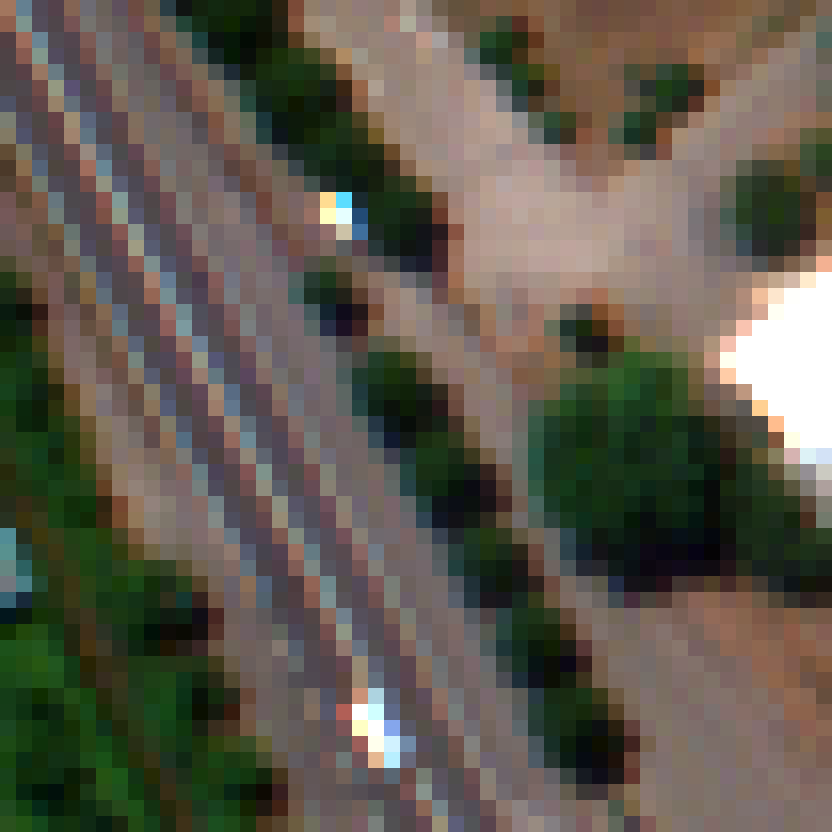
\includegraphics[width=6.5cm]{figures/pavia_patch.png}};
  \draw[pmuted!70, thin] (7.15,0) rectangle (20.15,13);
  % marked background pixel + halo
  \draw[pyellow, line width=1.0pt] (12.90,7.00) rectangle (13.15,7.25);
  \draw[pyellow, line width=0.6pt, dashed] (12.40,6.50) rectangle (13.65,7.75);
  % zoom lines down to the spectrum panel
  \draw[white, line width=2.3pt] (12.40,6.50) -- (1.40,-2.20);
  \draw[white, line width=2.3pt] (13.65,6.50) -- (25.90,-2.20);
  \draw[pyellow, line width=1.3pt] (12.40,6.50) -- (1.40,-2.20);
  \draw[pyellow, line width=1.3pt] (13.65,6.50) -- (25.90,-2.20);
  % ---- spectrum panel (below the image)
  \begin{scope}[shift={(1.4,-8.2)}]
    \draw[pmuted!60, line width=0.6pt] (0,0) -- (24.5,0);
    \draw[pmuted!60, line width=0.6pt] (0,0) -- (0,6.0);
    \draw[pnavy, line width=0.9pt] plot coordinates
      {(0.00,1.35) (0.47,0.79) (0.96,0.69) (1.43,0.71) (1.93,0.66) (2.40,0.59) (2.89,0.60) (3.36,0.54) (3.83,0.54) (4.33,0.56) (4.80,0.60) (5.29,0.66) (5.76,0.72) (6.26,0.80) (6.72,0.85) (7.19,0.88) (7.69,0.88) (8.16,0.81) (8.65,0.78) (9.12,0.70) (9.62,0.71) (10.09,0.68) (10.56,0.66) (11.05,0.65) (11.52,0.62) (12.02,0.61) (12.48,0.60) (12.98,0.58) (13.45,0.54) (13.94,0.54) (14.41,0.54) (14.88,0.54) (15.38,0.56) (15.85,0.70) (16.34,1.01) (16.81,1.50) (17.31,2.01) (17.78,2.69) (18.24,3.33) (18.74,3.76) (19.21,4.10) (19.70,4.14) (20.17,4.06) (20.67,4.21) (21.14,4.19) (21.61,4.12) (22.10,4.10) (22.57,4.10) (23.07,3.94) (23.54,3.96) (24.03,3.81) (24.50,3.94)};
    \draw[pbrown, line width=0.9pt] plot coordinates
      {(0.00,3.17) (0.47,3.39) (0.96,3.89) (1.43,4.21) (1.93,4.44) (2.40,4.71) (2.89,4.86) (3.36,4.99) (3.83,5.05) (4.33,5.05) (4.80,5.02) (5.29,4.96) (5.76,4.92) (6.26,4.88) (6.72,4.71) (7.19,4.60) (7.69,4.42) (8.16,4.25) (8.65,4.05) (9.12,3.80) (9.62,3.50) (10.09,3.19) (10.56,2.97) (11.05,2.81) (11.52,2.69) (12.02,2.60) (12.48,2.56) (12.98,2.50) (13.45,2.46) (13.94,2.48) (14.41,2.51) (14.88,2.59) (15.38,2.62) (15.85,2.68) (16.34,2.73) (16.81,2.73) (17.31,2.66) (17.78,2.59) (18.24,2.61) (18.74,2.66) (19.21,2.75) (19.70,2.78) (20.17,2.76) (20.67,2.80) (21.14,2.78) (21.61,2.80) (22.10,2.82) (22.57,2.90) (23.07,2.95) (23.54,3.01) (24.03,3.06) (24.50,3.15)};
    % target-pixel example: w + 0.15 s (dashed)
    \draw[pteal, line width=0.9pt, dashed] plot coordinates
      {(0.00,1.80) (0.47,1.27) (0.96,1.25) (1.43,1.31) (1.93,1.30) (2.40,1.27) (2.89,1.30) (3.36,1.26) (3.83,1.27) (4.33,1.29) (4.80,1.32) (5.29,1.38) (5.76,1.43) (6.26,1.50) (6.72,1.53) (7.19,1.54) (7.69,1.51) (8.16,1.42) (8.65,1.36) (9.12,1.24) (9.62,1.21) (10.09,1.13) (10.56,1.08) (11.05,1.04) (11.52,1.00) (12.02,0.97) (12.48,0.96) (12.98,0.93) (13.45,0.88) (13.94,0.88) (14.41,0.89) (14.88,0.90) (15.38,0.92) (15.85,1.07) (16.34,1.39) (16.81,1.88) (17.31,2.38) (17.78,3.05) (18.24,3.69) (18.74,4.13) (19.21,4.48) (19.70,4.53) (20.17,4.45) (20.67,4.60) (21.14,4.58) (21.61,4.51) (22.10,4.49) (22.57,4.51) (23.07,4.35) (23.54,4.38) (24.03,4.24) (24.50,4.38)};
    \node[fill=white, inner sep=1pt, text=pnavy, anchor=west] at (17.6,0.58) {background $w$};
    \node[text=pteal, anchor=south east] at (24.3,4.72) {target pixel $= w + 0.15\, s$};
    \node[text=pbrown, anchor=south west] at (6.0,5.35) {$s$ -- known target spectrum};
    \node[text=pbody, anchor=north] at (12.25,-0.30) {spectral band $1,\ldots,d$};
  \end{scope}
\end{tikzpicture}
\caption{The additive model on real data. Top: a pseudo-color patch of the
Pavia University scene, where each pixel is a $103$-dimensional spectral
vector. Bottom: the spectrum $w$ of the marked background pixel, the known
target spectrum $s$, and the resulting weak target pixel $w+0.15\,s$.}
\label{fig:pavia_patch}
\end{figure}



The classical large-sample tests for a composite scalar-parameter problem are the
\emph{Rao} test, the \emph{Wald} test, and the \emph{generalized
likelihood ratio test} (GLRT) --- the dominant family in adaptive
detection~\cite{kelly1986adaptive,robey1992cfar,kraut2001adaptive,vinGRLT}.
Under standard regularity conditions, these tests are asymptotically
equivalent~\cite{kay1998detection}. In this work, we focus on the LMP test,
which in our setting coincides with the one-sided Rao
test~\cite{rao1948large}, for its compatibility with score-based background
learning~\cite{kay1989asymptotically,demaio2007rao}:


Let $p_y(y;\theta)$ denote the likelihood under amplitude $\theta$, and define
\begin{align}
    u(y; \theta)
    &= \frac{\partial}{\partial \theta} \ln p_y(y;\theta), \nonumber\\
    I(\theta)
    &= \E_\theta\!\left[u^2(y;\theta)\right],
\end{align}
the score and Fisher information with respect to $\theta$. The LMP detector is
\begin{align}
    T_{\mathrm{LMP}}(y)
    &= \frac{u(y;\,0)}{\sqrt{I(0)}}.
    \label{eq:lmp_general}
\end{align}
Under $\Hnull$, $T_{\mathrm{LMP}}$ has zero mean and unit variance by
construction; asymptotic normality holds in the classical regime of many
i.i.d.\ observations~\cite{kay1998detection}, which we do not rely on here.
% Under $\Hnull$, $T_{\mathrm{LMP}}$ is asymptotically distributed as $\N(0,1)$. 
In the  additive noise formulation of~(\ref{eq:additive_model}), the test reduces to
\begin{align}
    T_{\mathrm{LMP}}(y)
    &= \frac{-s^\top \score(y)}{\sqrt{s^\top \Psi\, s}}.
    \label{eq:lmp_additive}
\end{align}
so the detector depends on the background only through the score and its covariance:
\begin{align}
    \score(w) &= \nabla_w \log p_w(w), \nonumber\\
    \Psi &= \E\left[\score(w)\score^\top(w)\right].
    \label{eq:fi_add}
\end{align}
\chapter{Score Matching Based Detection}
\label{score_matching_detection}
\label{sec:score_matching_detection}
We now turn to the main methodological step: estimating the background score from target-free secondary data and plugging it into the LMP detector. Let
\begin{equation}
    w_1,\ldots,w_n \overset{\mathrm{i.i.d.}}{\sim} p_w
\end{equation}
denote the secondary samples.

To estimate the background score without evaluating the normalizing constant of $p_w$, we can use implicit score matching (ISM) introduced by Hyv\"arinen~\cite{hyvarinen2005estimation}:
\begin{equation}
    \min_\eta \frac{1}{n} \sum_i \left[
        \tfrac{1}{2}\|\score_\eta(w_i)\|^2
        + \operatorname{tr}\!\bigl(\nabla_w \score_\eta(w_i)\bigr)
    \right].
\end{equation}
This objective contains the divergence term, i.e. the trace of the Jacobian of $\score_\eta$, which is costly to evaluate and back-propagate through for neural models. We therefore turn to
\emph{denoising} score matching (DSM)~\cite{vincent2011connection},
which replaces that term by a Gaussian-perturbation regression with a fixed corruption
level $\sigma>0$. For each secondary sample we draw a corrupted copy
\begin{align}
    \tilde w_i &= w_i + \sigma\varepsilon_i,
    \nonumber\\
    \varepsilon_i&\sim \N(0,I_d),
\end{align}
and train $\score_\eta:\R^d\to\R^d$ by minimizing
\begin{equation}
    \hat\eta
    = \arg\min_\eta
    \frac1n\sum_{i=1}^n
    \left\|
    \score_\eta(\tilde w_i) - \frac{w_i-\tilde w_i}{\sigma^2}
    \right\|^2.
    \label{eq:DART_objective}
\end{equation}
The regression target $(w_i-\tilde w_i)/\sigma^2$ is the analytic score of the Gaussian
corruption kernel. At the population optimum,
\begin{align}
    \score_{\eta^*}(x)
    &= \nabla_x \log q_\sigma(x)\nonumber\\
    q_\sigma &= p_w * \mathcal{N}(0,\sigma^2 I_d),
\end{align}
so $\score_{\hat\eta}$ estimates the score of the noise-smoothed density $q_\sigma$, and
tends to $\nabla\log p_w$ as $\sigma\to0$ (Tweedie's formula~\cite{efron2011tweedie}%
). 

The noise level $\sigma$ governs a bias-variance tradeoff: a small $\sigma$ keeps $q_\sigma$ close to $p_w$, while a larger one stabilizes estimation and keeps the score informative away from the training samples.
Motivated by the analogy with kernel bandwidth selection~\cite{silverman1986density}, we set $\sigma$ proportional to the empirical RMS scale of the data, $\sigma^2 = \rho\,\hat{s}^2$ with $\hat{s}^2 = \operatorname{tr}(\widehat{\Sigma}_n)/d$, where $\widehat{\Sigma}_n$ is the empirical covariance of the background samples, computed in the normalized coordinates on which the score network operates.
The dimensionless factor $\rho$ is small, so $\sigma$ remains well below the data scale, and decreases as the number of secondary samples grows, just as a kernel bandwidth narrows with sample size.
After learning the score, we estimate the score covariance from the same secondary samples:
\begin{align}
    \widehat{\Psi}
    = \frac{1}{n}\sum_{i=1}^n
    \score_{\hat\eta}(w_i)\score_{\hat\eta}(w_i)^\top.
    \label{eq:psi_hat}
\end{align}
This yields the proposed DART detector
\begin{align}
    \widehat T_{\mathrm{DART}}(y)
    = \frac{-s^\top \score_{\hat\eta}(y)}
    {\sqrt{s^\top \widehat{\Psi}\, s}}.
    \label{eq:lmp_plugin}
\end{align}
While the ideal statistic is standardized under $\Hnull$, the null distribution of the plug-in statistic with a learned score is unknown, and its asymptotic normality cannot be established. We therefore set detection thresholds empirically, from an upper quantile of the statistic evaluated on the target-free secondary samples, $\{\widehat T_{\mathrm{DART}}(w_i)\}_{i=1}^n$.
The complete learning and test procedure is summarized in Fig.~\ref{fig:dart_pipeline}.

% Adapted from the MLSP 2026 poster (column 2): the DART pipeline at
% learning time and at test time.
\begin{figure}[htbp]
\centering
\resizebox{\textwidth}{!}{%
\begin{tikzpicture}[x=0.5cm, y=0.5cm, line cap=round, font=\footnotesize\linespread{1}\selectfont,
  dbox/.style={draw=pmuted!60, fill=white, rounded corners=1mm, line width=0.5pt,
               align=center, inner sep=1.3mm},
  darr/.style={-stealth, line width=0.7pt, pnavy!75}]
  % ================= LEARNING TIME =================
  \draw[pnavy!70, dashed, line width=0.6pt, rounded corners=1.5mm] (0,6.3) rectangle (27.2,11.4);
  \node[anchor=north west, font=\footnotesize\bfseries, text=pnavy] at (0.4,11.2) {Learning time};
  \node[dbox, anchor=west] (n1) at (2.3,8.3) {target-free\\ $w_1,\ldots,w_n \overset{\text{iid}}{\sim} p_w$};
  \node[dbox, right=0.6cm of n1] (n2) {score net $\psi_\eta$\\ DSM training};
  \node[dbox, right=0.6cm of n2] (n3) {statistics\\ $\widehat{T}_{\mathrm{DART}}(w_i)$};
  \node[dbox, right=0.6cm of n3] (n4) {threshold\\ $\gamma = \hat{q}_{\,1-\alpha}$};
  \draw[darr] (n1) -- (n2);
  \draw[darr] (n2) -- (n3);
  \draw[darr] (n3) -- (n4);
  % ================= TEST TIME =================
  \draw[pbrown!75, dashed, line width=0.6pt, rounded corners=1.5mm] (0,-0.1) rectangle (27.2,4.9);
  \node[anchor=north west, font=\footnotesize\bfseries, text=pbrown] at (0.4,4.7) {Test time};
  \node[dbox] (m4) at (n4.center |- 0,2.1) {declare $\Halt$ if\\ $\widehat{T}_{\mathrm{DART}}(y) \gtrless \gamma$};
  \node[dbox, left=0.6cm of m4] (m3) {statistic\\ $\widehat{T}_{\mathrm{DART}}(y)$};
  \node[dbox, left=0.6cm of m3] (m2) {score net $\psi_{\hat\eta}$\\ (frozen)};
  \node[dbox, left=0.6cm of m2] (m1) {test pixel\\ $y_i$};
  \draw[darr] (m1) -- (m2);
  \draw[darr] (m2) -- (m3);
  \draw[darr] (m3) -- (m4);
  % gamma feeds the test-time decision
  \draw[darr] (n4.south) -- (m4.north);
  \node[text=pnavy, anchor=west] at ([shift={(0.3,-1.2)}]n4.south) {$\gamma$};
\end{tikzpicture}}
\caption{The DART pipeline. At learning time the score network is trained
on the target-free secondary samples with the DSM objective
\eqref{eq:DART_objective}, the statistic $\widehat{T}_{\mathrm{DART}}$ is
evaluated on the same samples, and the detection threshold $\gamma$ is set
to its empirical upper quantile. At test time the frozen network is applied
to each pixel and the statistic \eqref{eq:lmp_plugin} is compared with
$\gamma$.}
\label{fig:dart_pipeline}
\end{figure}


\section{Special case: Gaussian background}
\label{sec:special}

The Gaussian case makes the role of score matching explicit. Suppose
$
w \sim \mathcal{N}(\mu,\Sigma)
$
and restrict the score model to the affine class
$
\psi_\eta(w)=A(w-\mu).
$
Since
\begin{equation}
\psi(w)=-\Sigma^{-1}(w-\mu),
\end{equation}
the affine class is correctly specified.

\noindent\textbf{ISM.}
Minimizing the implicit score-matching objective over the affine class recovers
the empirical Gaussian score ~\cite{hyvarinen2005estimation}:
\begin{equation}
\hat\psi_{\mathrm{ISM}}(y)=-\hat\Sigma_n^{-1}(y-\hat\mu_n),
\end{equation}
where $\hat\mu_n$ and $\hat\Sigma_n$ are the sample mean and covariance.
Substituting this into the plug-in LMP statistic yields the usual Gaussian
matched-filter form, i.e. the adaptive matched filter (AMF) ~\cite{robey1992cfar,kelly1986adaptive}.

\noindent\textbf{DSM.}
Denoising score matching estimates the score of the smoothed density
$
q_\sigma = p_w * \mathcal{N}(0,\sigma^2 I)
$
rather than that of $p_w$ itself \cite{vincent2011connection}. Equivalently,
\begin{equation}
\nabla_{\tilde w}\log q_\sigma(\tilde w)
=
\frac{\mathbb{E}[w\mid \tilde w]-\tilde w}{\sigma^2},
\label{eq:tweedie}
\end{equation}
which expresses the score in terms of the posterior mean under Gaussian
corruption \cite{efron2011tweedie}. For Gaussian clutter,
\begin{equation}
    q_\sigma=\mathcal{N}(\mu,\Sigma+\sigma^2 I)
\end{equation}
hence
\begin{equation}
\hat\psi_{\mathrm{DSM}}(y)
=
-(\hat\Sigma_n+R_n)^{-1}(y-\hat\mu_n+r_n).
\label{eq:gauss_DART_solution0}
\end{equation}
where $R_n$ and $r_n$ are empirical moments of the noise. Asymptotically, these residual moments vanish and the DSM score converges to
\begin{equation}
\hat\psi_{\mathrm{DSM}}(y)
\rightarrow
-(\hat\Sigma_n+\sigma^2 I)^{-1}(y-\hat\mu_n).
\label{eq:gauss_DART_solution}
\end{equation}
Thus, in the affine Gaussian setting, DSM replaces the inverse sample
covariance by a diagonally loaded inverse covariance. In adaptive detection,
this is the classical regularization used to stabilize matched-filter
statistics when $\hat\Sigma_n$ is ill-conditioned or the number of secondary
samples is small ~\cite{carlson1988covariance}. This connection explains the improved
small-sample robustness of linear DART in our experiments.

\chapter{Spatially Adapted Detector}
\label{sec:spatial_score_matching}

In hyperspectral and radar detection the background is often only locally
homogeneous, and the most informative secondary samples for calibration are
the neighboring target-free cells rather than draws from the full scene.
DARTS, developed next, adapts the denoising detector to this setting.

Let $\Omega$ denote the set of image pixels and let $y_i \in \mathbb{R}^d$ be the
spectral vector at pixel $i \in \Omega$. For each pixel, let
$\mathcal{A}_i$ denote a local neighborhood. We define a conditional score
estimator
\begin{equation}
\widehat{\psi}_i(y_i)
=
\widehat{\psi}_{\eta}
\left(
y_i;\{y_j : j \in \mathcal{A}_i\}
\right),
\label{eq:local_score_estimator}
\end{equation}
where $\eta$ are learned parameters. We instantiate $\widehat{\psi}_i$ with a
shared multilayer perceptron (MLP) encoder that embeds the center pixel and each pixel in its local
window into a low-dimensional latent space. The $K$ nearest neighbors in latent
Euclidean distance are pooled into a context feature, which is concatenated with
the center embedding and decoded by a second MLP into the score. As before, the
model is trained on denoising residuals, with noise added only to the test
pixel. The encoder and the score head are trained jointly by minimizing this
single DSM objective end to end; no auxiliary loss is used to shape the latent
space. The architecture and the resulting pipeline are shown in Fig.~\ref{fig:darts-architecture}.

% Adapted from the MLSP 2026 poster (column 3): the DARTS architecture and
% pipeline.  Replaces Fig. 1 (fig:darts-architecture) of the MLSP paper.
\begin{figure}[htbp]
\centering
\resizebox{\textwidth}{!}{%
\begin{tikzpicture}[x=0.5cm, y=0.5cm, line cap=round, font=\footnotesize\linespread{1}\selectfont,
  dbox/.style={draw=pmuted!60, fill=white, rounded corners=1mm, line width=0.5pt,
               align=center, inner sep=1.2mm},
  cnet/.style={draw=pmuted!50, fill=white, rounded corners=1.5mm, line width=0.55pt,
               align=center, inner sep=1.2mm},
  darr/.style={-stealth, line width=0.7pt, pnavy!75}]
  % ================= LEARNING TIME =================
  \draw[pnavy!70, dashed, line width=0.6pt, rounded corners=1.5mm] (0,6.8) rectangle (27.2,22.4);
  \node[anchor=north west, font=\footnotesize\bfseries, text=pnavy] at (0.4,22.2) {Learning time};
  % k x k neighbourhood grid
  \begin{scope}[shift={(1.2,16.4)}]
    \foreach \x in {0,...,6} \foreach \y in {0,...,6}
      \draw[pmuted!45, line width=0.3pt] (\x*0.6,\y*0.6) rectangle (\x*0.6+0.6,\y*0.6+0.6);
    \foreach \x/\y in {1/5, 5/5, 1/1, 5/2, 0/3, 3/6}
      \fill[pbrown!32] (\x*0.6+0.03,\y*0.6+0.03) rectangle (\x*0.6+0.57,\y*0.6+0.57);
    \fill[pnavy] (3*0.6+0.03,3*0.6+0.03) rectangle (3*0.6+0.57,3*0.6+0.57);
  \end{scope}
  % legend: center pixel + neighbourhood definition
  \node[anchor=north west, align=left, font=\scriptsize, text=pbody] at (0.9,10.2)
    {\textcolor{pnavy}{$\blacksquare$}\ $w_i$ -- center pixel\\[0.3mm]
     \textcolor{pbrown!70}{$\blacksquare$}\ $\{w_j\}_{j \in \mathcal{A}_i}$ -- local window};
  % ---- cond. net container ----
  \draw[pmuted!50, line width=0.55pt, rounded corners=1.5mm] (6.8,10.8) rectangle (26.8,21.2);
  \node[anchor=north west, font=\footnotesize\bfseries, text=pmuted] at (7.15,20.95) {cond.\ net $\widehat{\psi}_i$};
  \node[dbox] (enc)  at (11.9,18.4) {shared encoder $e_\eta$\\ $z_i = e_\eta(w_i),\ z_j = e_\eta(w_j)$};
  \node[dbox] (pool) at (21.9,18.4) {$K$-NN in latent space\\ pooled context $c_i$};
  \node[dbox] (sc)   at (16.8,12.9) {score head (MLP)\\ $\widehat{\psi}_i = \psi_\eta(w_i,\, z_i,\, c_i)$};
  \draw[darr] (5.4,18.4) -- (enc.west);
  \draw[darr] (enc) -- (pool);
  % z_i and c_i drop into the score head (right angles, separate entry points)
  \draw[darr] (enc.south) -- ++(0,-1.6) -| ([xshift=-0.67cm]sc.north);
  \node[font=\scriptsize, text=pnavy, anchor=west] at ([shift={(0.22,-0.75)}]enc.south) {$z_i$};
  \draw[darr] (pool.south) -- ++(0,-2.6) -| ([xshift=+0.67cm]sc.north);
  \node[font=\scriptsize, text=pnavy, anchor=west] at ([shift={(0.22,-0.75)}]pool.south) {$c_i$};
  % raw center pixel skip
  \draw[darr] (5.0,16.4) |- (sc.west);
  \node[font=\scriptsize, text=pbrown, anchor=south west] at (5.6,13.05) {$w_i$};
  % ---- statistics -> threshold (below the container) ----
  \node[dbox] (st) at (16.8,8.7) {statistic $\widehat{T}_i^{\,\mathrm{DARTS}}(w_i)$};
  \node[dbox, right=0.55cm of st] (ga) {$\gamma = \hat{q}_{\,1-\alpha}$};
  \draw[darr] (sc.south) -- (st.north);
  \draw[darr] (st) -- (ga);
  % ================= TEST TIME =================
  \draw[pbrown!75, dashed, line width=0.6pt, rounded corners=1.5mm] (0,0.0) rectangle (27.2,5.6);
  \node[anchor=north west, font=\footnotesize\bfseries, text=pbrown] at (0.4,5.4) {Test time};
  \node[dbox, anchor=west] (m1) at (1.0,2.5) {pixel + nbhd\\ $y_i,\ \{y_j\}_{j\in\mathcal{A}_i}$};
  \node[cnet, right=0.46cm of m1] (m2) {cond.\ net $\widehat{\psi}_i$\\ (frozen)};
  \node[dbox, right=0.46cm of m2] (m3) {statistic\\ $\widehat{T}_i^{\,\mathrm{DARTS}}(y_i)$};
  \node[dbox, right=0.46cm of m3] (m4) {declare $\Halt$ if\\ $\widehat{T}_i^{\,\mathrm{DARTS}} \gtrless \gamma$};
  \draw[darr] (m1) -- (m2);
  \draw[darr] (m2) -- (m3);
  \draw[darr] (m3) -- (m4);
  % gamma feeds the test-time decision (right angles, jog in the gap)
  \draw[darr] (ga.south) -- ++(0,-2.1) -| (m4.north);
  \node[text=pnavy, anchor=west] at ([shift={(0.2,-1.7)}]ga.south) {$\gamma$};
\end{tikzpicture}}
\caption{DARTS architecture and pipeline. A shared encoder $e_\eta$ maps the
center pixel and the pixels of its local window $\mathcal{A}_i$ to
low-dimensional latents. The $K$ nearest neighbor latents are pooled into a
local context vector $c_i$, and the score head receives the raw center
pixel, its latent $z_i$, and $c_i$. The conditional network is trained end
to end with the single DSM objective; the locally normalized statistic
\eqref{eq:local_normalized_rao_vector} evaluated on the target-free
secondary pixels sets the threshold $\gamma$, which is then applied to the
test pixels.}
\label{fig:darts-architecture}
\end{figure}


At test time, DARTS plugs the neighbor-conditioned score into the LMP statistic. It is designed for heterogeneous background and we therefore normalize it using local score covariances
\begin{equation}
\widehat{T}_i^{\,\mathrm{DARTS}}
=\frac{-s^\top\!\left(\widehat{\psi}_i(y_i)-\widehat{m}_{\psi,i}\right)}
      {\sqrt{s^\top \widetilde{\Psi}_i\, s+\epsilon}},
\label{eq:local_normalized_rao_vector}
\end{equation}
where 
\begin{align}
\widehat{m}_{\psi,i}&=\frac{1}{|\mathcal{A}_i|}\sum_{j\in\mathcal{A}_i}
\widehat{\psi}_j(y_j),\nonumber\\
\widehat{\Psi}_i&=\frac{1}{|\mathcal{A}_i|}\sum_{j\in\mathcal{A}_i}
\left(\widehat{\psi}_j(y_j)-\widehat{m}_{\psi,i}\right)
\left(\widehat{\psi}_j(y_j)-\widehat{m}_{\psi,i}\right)^{\!\top},
\label{eq:local_score_covariance}
\end{align}
and $\epsilon>0$ is a small numerical floor. In practice, the local covariance
estimate can be noisy when only a limited number of reliable neighbors is
available, so we regularize it toward the global score covariance:
\begin{equation}
\widetilde{\Psi}_i
=
(1-\lambda)\widehat{\Psi}_i+\lambda\widehat{\Psi},
\qquad 0\leq\lambda\leq1.
\label{eq:shrunk_local_fisher}
\end{equation}
where $\hat{\Psi}$ is defined in (\ref{eq:psi_hat}).

% \chapter{Research Question}
\label{chap:rq}


% \chapter{Methods}
\label{chap:methods}


\chapter{Experiments}
\label{sec:experiments}
% ============================================================
We evaluate the proposed DART(S) detectors on three real hyperspectral
scenes: the Pavia University dataset~\cite{paviau_gic}, a $610\times340$
scene with 103 spectral bands and nine labeled land-cover classes plus an
unlabeled background, the San Diego I airport image, a $100\times100$ scene
with 189 spectral bands containing real aircraft, and the Salinas scene \cite{salinas_data},
$512\times217$ with 204 spectral bands and sixteen labeled crop classes.
Hyperspectral data are severely ill-conditioned: training score networks
directly on raw spectra failed, full whitening amplifies the near-null
spectral directions by orders of magnitude and flattens the multimodal
structure the learned score relies on, and dimensionality reduction such as
PCA may discard directions containing the unknown target signature. On
every scene we therefore normalize the inputs of the proposed detectors
with a fixed shrinkage whitening $W=(R+\lambda_w I)^{-1/2}D^{-1/2}$
estimated from the training background, where $D$ and $R$ are the variances
and the correlation matrix of the secondary samples and $\lambda_w=2$. It
preserves the original dimension and decorrelates only mildly, which
conditions the optimization while keeping that structure intact.


\section{IID background}
\label{sec:exp-iid}

To approximate the i.i.d.\ setting of Section~\ref{sec:score_matching_detection}, we sample background pixels at random from one or more labeled classes, split them into disjoint training and test sets, and plant a class-mean signature $s$ in a random fraction of the test pixels under the additive model~\eqref{eq:additive_model} with $\theta=0.15$.
We compare AMF~\cite{robey1992cfar,kelly1986adaptive}, GMM-Levin~\cite{levin2019cluster}, LRao~\cite{lrao2026}, and our DART detector. LRao is trained with its published signal-aware objective and robust input normalization, with a score network matched to DART's architecture.

% Fig. 2 of the MLSP paper (figures/iid_grid.pdf).  The paper shows the
% four panels in one wide strip; on an A4 page the strip is split, as on
% the poster, into the legend, the P_d-versus-n pair and the rho-sweep pair
% (the trim values crop the single PDF).
\begin{figure}[htbp]
\centering
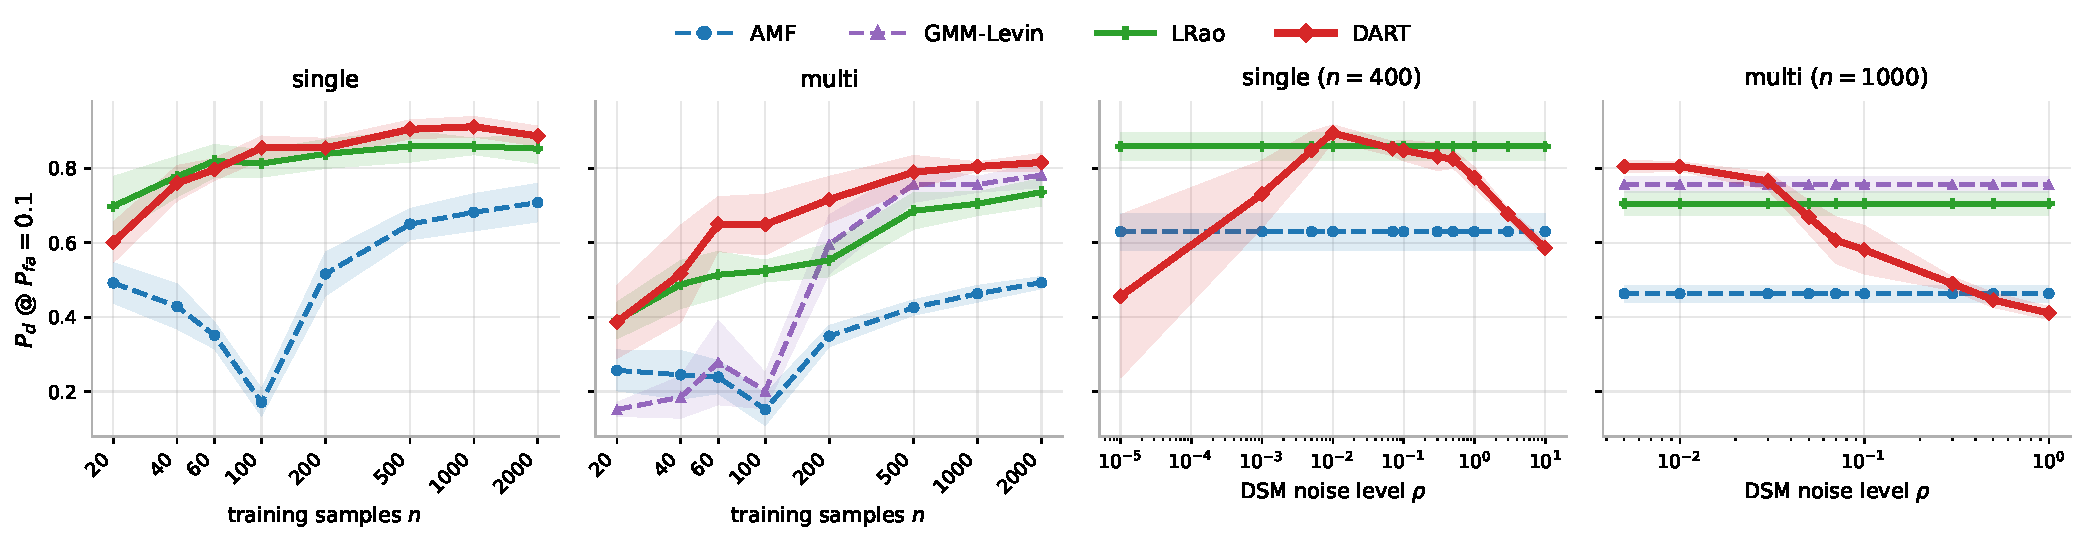
\includegraphics[width=0.55\textwidth, trim=322 238.8 322 9, clip]{figures/iid_grid.pdf}\\[2mm]
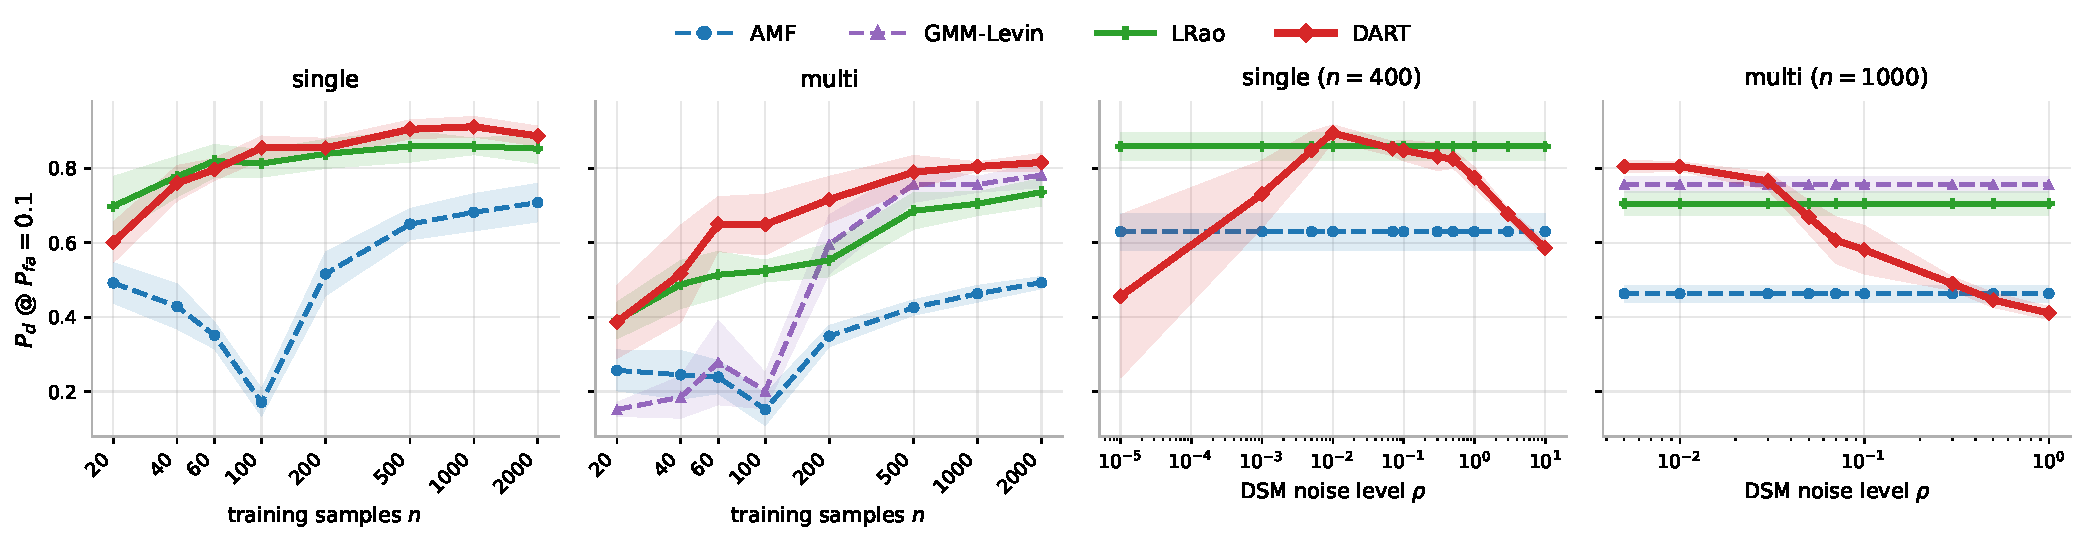
\includegraphics[width=\textwidth, trim=4.8 5.6 487.4 30.4, clip]{figures/iid_grid.pdf}\\[3mm]
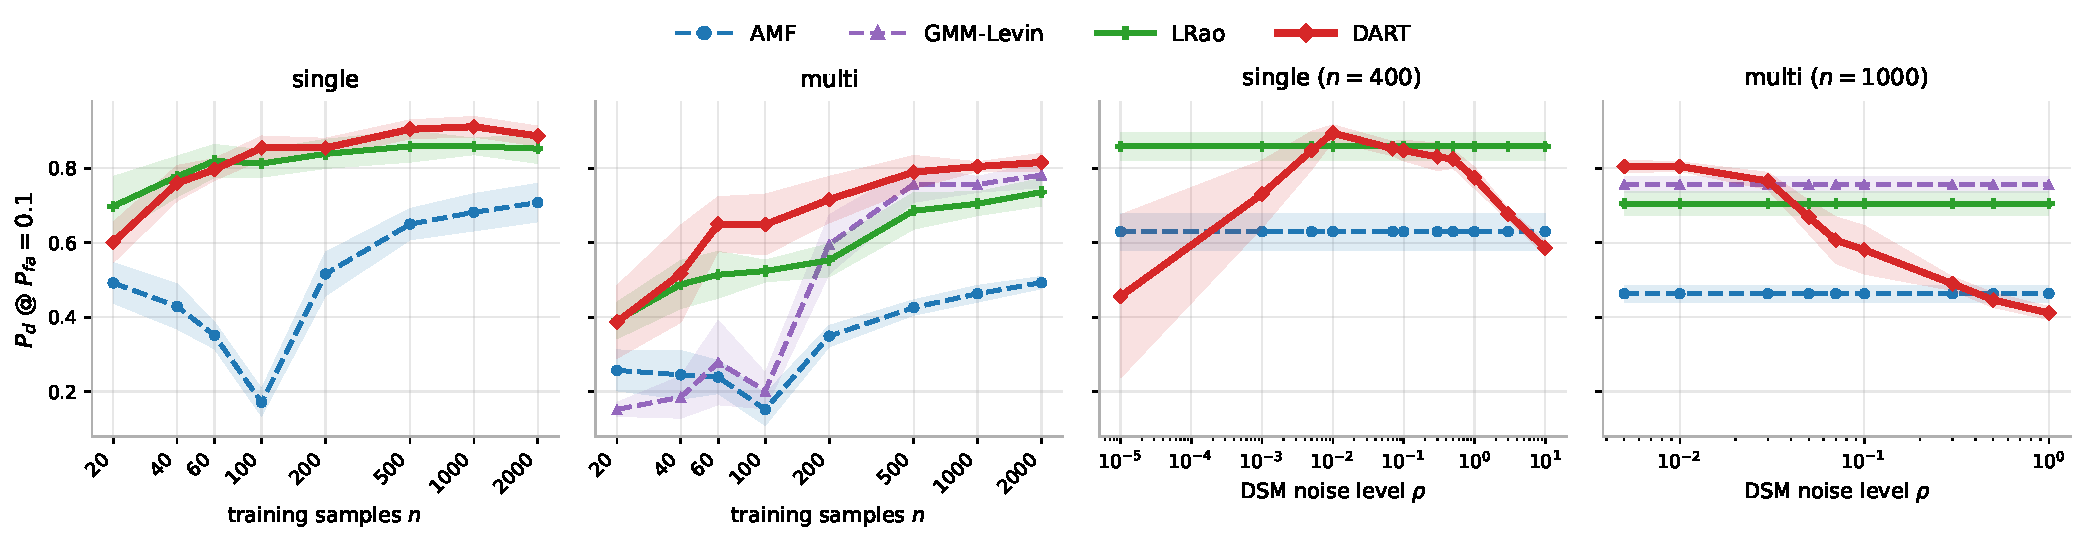
\includegraphics[width=\textwidth, trim=517 5.6 2 30.4, clip]{figures/iid_grid.pdf}
\caption{IID experiments on Pavia University ($5$ seeds, $\pm1\sigma$
bands). \emph{Top row}: $P_d$ at $P_{fa}=0.1$ versus the number of
secondary samples $n$ for the single-class and multi-class backgrounds;
the unregularized AMF collapses near $n\approx d$, where the sample
covariance is rank deficient, whereas the learned detectors are unaffected;
for DART this stability comes from the implicit loading supplied by the DSM
noise. \emph{Bottom row}:
robustness to the DSM noise level $\rho$ at fixed $n$. On the single-class
background, performance is flat over a wide plateau spanning
$\rho\in[5\!\times\!10^{-3},5\!\times\!10^{-1}]$; on the multi-class
background it peaks at small $\rho$ and degrades monotonically as the
blur washes out the mixture structure DART exploits. The operating point
$\rho=0.01$, used in the IID experiments, sits at the optimum in
both cases ($\rho$-independent detectors are drawn as flat references).}
\label{fig:ablation_single}
\label{fig:ablation_multi}
\end{figure}


The first simulation draws the background from a single labeled class, which makes the comparison with the AMF most direct and isolates the regularizing effect of denoising. The first panel of Fig.~\ref{fig:ablation_single} agrees with the Gaussian special case of Section~\ref{sec:special}: the AMF degrades sharply as $n$ approaches the ambient dimension, whereas the implicitly loaded DART is unaffected. LRao is the most effective detector at the smallest sample sizes, and DART leads beyond roughly one hundred samples.

The second simulation combines pixels from six labeled classes into a proportionally mixed background, shifting the emphasis from small-sample stability to the expressive power of the learned score under model mismatch (second panel). DART leads across nearly the entire range of $n$, as the learned score captures non-Gaussian structure that a single Gaussian cannot represent. LRao is the most effective of the remaining detectors at small and moderate sample sizes, and GMM-Levin, whose parametric mixture is well matched to this background, overtakes it at larger $n$.


\section{Correlated background}
\label{sec:spatial}

We now turn to a more realistic setting and evaluate DARTS on Pavia
University, San Diego I, and Salinas. For each scene, we use spatially disjoint training and test boxes, plant targets under the additive model in $10\%$ of the test pixels, and compare local AMF, GMM-Levin, and LRao against the spatially adapted DARTS ($\lambda=0.1$, with a $7\times 7$
neighborhood and $K=7$ pooled neighbors), together with four recent deep detectors, OS-VAE ~\cite{osvae}, HTD-Net ~\cite{htd-net}, THANTD ~\cite{thantd}, and TSTTD ~\cite{tsttd}, each first validated at its published performance on its own benchmark and then trained with its own recipe from the same prior signature and target-free
secondary pixels.
In our runs these baselines were not competitive in this regime and are
therefore omitted from the tables; we defer their detailed treatment to
future work.
As ablations we vary the two ingredients of DARTS in turn
(Table~\ref{tab:spatial}, lower block): the conditioning of the score, by
inserting the unconditioned DART score into the normalized
statistic~\eqref{eq:local_normalized_rao_vector}, and the shrinkage
$\lambda$ of the local score covariance toward the global one. Removing
both recovers the global DART detector.
LRao is trained as its authors prescribe, with early stopping on a held-out validation cost;
the 20\% validation split leaves it fewer secondary pixels than the other
detectors. We report the area under the ROC curve (AUC), the partial AUC
over false alarm rates below $0.05$ (pAUC$_{0.05}$), the detection rate at
a $0.05$ false alarm rate ($P_d@0.05$), and empirical false alarm rates
$\hat P_{fa}$ at thresholds set from the training background scores.

% Table 1 of the MLSP paper (tab:spatial), verbatim.
\begin{table}[htbp]
\centering
\caption{Spatial detection on the correlated Pavia-U scene ($\theta=0.15$,
5 seeds). $\hat P_{fa}^{\max}$ is the largest per-class false alarm rate at
a threshold set to the empirical $0.05$ upper quantile of the training
background scores; the nominal level is $0.05$. Bold marks the best value
within each block. The ablations vary two ingredients of DARTS
independently: whether the score in
Eq.~\eqref{eq:local_normalized_rao_vector} is conditioned on the
neighboring pixels, and the shrinkage $\lambda$ of the local score
covariance toward the global one in
Eq.~\eqref{eq:shrunk_local_fisher}. A dash in the $\lambda$ column
indicates that no local score normalization is applied.}
\label{tab:spatial}
\small
\setlength{\tabcolsep}{5pt}
\renewcommand{\arraystretch}{1.15}
\begin{tabular}{@{}lc ccc c@{}}
\toprule
 & & \multicolumn{3}{c}{Detection} & Calibration\\
\cmidrule(lr){3-5}\cmidrule(l){6-6}
Detector & $\lambda$ & pAUC$_{0.05}$ & AUC & $P_d@0.05$ & $\hat P_{fa}^{\max}$\\
\midrule
DARTS      & 0.1 & \textbf{0.556} & \textbf{0.926} & \textbf{0.730} & \textbf{0.088}\\
\addlinespace[2pt]
AMF        & --  & 0.238 & 0.786 & 0.346 & 0.103\\
GMM-Levin  & --  & 0.129 & 0.773 & 0.229 & 0.455\\
LRao       & --  & 0.137 & 0.713 & 0.220 & 0.761\\
\midrule
\multicolumn{6}{@{}l}{\emph{Ablations --- score conditioning and shrinkage $\lambda$:}}\\
\addlinespace[1pt]
\quad conditioned            & 0.9 & \textbf{0.533} & \textbf{0.925} & \textbf{0.728} & 0.066\\
\quad conditioned            & 1.0 & 0.525 & 0.924 & 0.726 & 0.062\\
\addlinespace[2pt]
\quad unconditioned          & 0.1 & 0.304 & 0.846 & 0.453 & 0.038\\
\quad unconditioned          & 0.9 & 0.311 & 0.846 & 0.443 & \textbf{0.019}\\
\quad unconditioned, no norm.\ & --  & 0.153 & 0.750 & 0.254 & 0.060\\
\bottomrule
\end{tabular}
\end{table}



On Pavia, DARTS attains the highest pAUC, AUC and $P_d$ among the methods
considered, and its largest per class false alarm rate is the closest to
the nominal level. The baselines rank lower, and under a single global
threshold their per class rates depart further from the nominal level.

The ablations isolate the contribution of each ingredient. Local
normalization is valuable on its own: inserting the unconditioned score
into the normalized statistic improves detection substantially over the raw
global statistic. Most of this gain persists when the local score
covariance is shrunk toward the global one, which suggests that the removal
of the local score mean accounts for much of the effect. Normalization
alone, however, is not sufficient. The unconditioned score remains well
below DARTS at matched $\lambda$, which indicates that the benefit of the
neighborhood lies in conditioning the learned score rather than in
correcting it after training. The value of $\lambda$ has only a minor
effect on detection and mainly governs the worst class false alarm rate.


% Table 2 of the MLSP paper (tab:sandiego), verbatim.  The paper sets it as
% a two-column table*; here the two scenes are stacked as two blocks so the
% table fits the A4 text width without shrinking.
\begin{table}[htbp]
\centering
\caption{Spatial detection at a common target amplitude $\theta=0.03$
(5 seeds): San Diego I with the real aircraft signature, Salinas with the
brocoli-green-weeds signature. DARTS uses local moment normalization
($\lambda=0.1$), AMF estimates its mean and covariance in a sliding window,
while GMM-Levin and LRao use their global statistics.}
\label{tab:sandiego}
\small
\setlength{\tabcolsep}{6pt}
\renewcommand{\arraystretch}{1.15}
\begin{tabular}{@{}l c cccc@{}}
\toprule
Detector & $\lambda$ & pAUC$_{0.05}$ & AUC & $P_d$@0.05 & $\hat P_{fa}$\\
\midrule
\multicolumn{6}{@{}l}{\emph{San Diego I}}\\
\addlinespace[1pt]
DARTS       & 0.1 & \textbf{0.634} & \textbf{0.956} & \textbf{0.791} & \textbf{0.020}\\
AMF         & --  & 0.361 & 0.919 & 0.607 & 0.054\\
GMM-Levin   & --  & 0.275 & 0.777 & 0.397 & 0.025\\
LRao        & --  & 0.177 & 0.776 & 0.276 & 0.041\\
\midrule
\multicolumn{6}{@{}l}{\emph{Salinas}}\\
\addlinespace[1pt]
DARTS       & 0.1 & 0.766 & \textbf{0.972} & \textbf{0.882} & \textbf{0.009}\\
AMF         & --  & \textbf{0.769} & 0.968 & 0.866 & 0.055\\
GMM-Levin   & --  & 0.038 & 0.864 & 0.062 & 0.132\\
LRao        & --  & 0.169 & 0.845 & 0.237 & 0.084\\
\bottomrule
\end{tabular}
\end{table}


Table~\ref{tab:sandiego} reports the same protocol on San Diego I and
Salinas. The target amplitude is reduced to $\theta=0.03$, where the scenes
remain challenging; at larger amplitudes the detectors saturate.
The results follow the same pattern, with DARTS comparing favorably on
both scenes. The local AMF is the strongest baseline here, and on Salinas,
whose large homogeneous fields are well matched to a local Gaussian model,
it comes close to DARTS. Amplitude sweeps and the reuse of a single learned
background model across additional target signatures are demonstrated in the
accompanying code repository.
% \chapter{Results}
\label{chap:results}

\chapter{Discussion and Future Work}
\label{chap:conclusion}
\label{sec:discussion}

We proposed DART, a denoising-score-assisted Rao detector that combines
classical weak-target detection with score-based background learning, and
its spatially adapted extension DARTS. The learned background model is
reusable across target signatures, and in the affine Gaussian case DART
reduces to a diagonally loaded adaptive matched filter, explaining its
finite-sample robustness.

Many directions remain open. First, stronger score-learning objectives may
improve detection; in particular, flow-matching or multi-noise
diffusion-style alternatives could learn more accurate scores. Second,
DARTS contains several manually selected hyperparameters, including the
network size, neighborhood size, number of neighbors, and
the shrinkage parameter $\lambda$; automatic tuning using only secondary
data is an important practical next step. Finally, robustness to target
leakage in the secondary data and a systematic ablation of the whitening
front-end remain to be studied.

Overall, DART shows that score-based learning can serve as a focused
replacement for the unknown background model inside a classical detector,
rather than as an end-to-end learned classifier, extending adaptive
detection beyond restrictive Gaussian assumptions while preserving
interpretability and calibration.


\bibliographystyle{apalike}
\bibliography{thesis}

\end{document}